\section{Progettazione}

\subsection{Design Persona}

Partendo dalla risorsa consigliata nel corso (\textit{Desining for Emotion} di
Aaron Walter), abbiamo descritto la personalità di partenza per sviluppare il
prodotto:

\begin{itemize}
	\item \textbf{Brand name}: a questo punto il nome del brand è noto, ovvero
	      \textit{Grigo Verde};

	\item \textbf{Overview}: il sito prosegue il lavoro degli studenti del Liceo
	      Grigoletti che hanno partecipato ad un progetto di riqualificazione
	      delle aree verdi della scuola. Per questo motivo il verde è il colore
	      predominante del sito;

	\item \textbf{Brand traits}:
	      \begin{itemize}
		      \item Formale ma non rigido: deve essere adatto ad un contesto
		            scolastico;
		      \item Simpatico ma non scherzoso: questo sito deve essere
		            consultato da dei docenti;
		      \item Schematico ma non povero;
		      \item Preciso: deve essere sempre pronto a rispondere ad ogni
		            esigenza dell'utente con la massima accuratezza.
	      \end{itemize}

	\item \textbf{Personality map}:
	      \begin{center}
		      \begin{tikzpicture}
			      \begin{axis}[
					      axis lines = middle,
					      xlabel = { amichevole },
					      ylabel = { formale },
					      xmin = -10, xmax = 10,
					      ymin = -10, ymax = 10,
					      xtick = {-10,-5,...,10},
					      ytick = {-10,-5,...,10},
				      ]
				      % template per mostrare il punto all'interno del piano cartesiano.
				      \addplot [
					      color=black,
					      mark=*,
					      only marks,
				      ] coordinates {
						      (3, 5)
					      } node[below] {$P$};
			      \end{axis}

		      \end{tikzpicture}
	      \end{center}

	\item \textbf{Visual lexicon}:
	      \begin{itemize}
		      \item \textbf{Colori}: verde scuro per i titoli, nero per i testi
		            e bianco per lo sfondo;
		      \item \textbf{Contorni}: arrotondati: la prenotazione delle
		            aule è una procedura precisa. Inserire dei contorni
		            arrotondati rende il prodotto più accattivante;
		      \item \textbf{Ombre}:assenti;

		      \item \textbf{Font}: \textit{Sans-Serif Arial};
	      \end{itemize}

	\item \textbf{Engagement methods}:
	      \begin{itemize}
		      \item \textbf{Design pulito e intuitivo}: l'utente deve essere in
		            grado di capire cosa fare senza dover leggere alcun manuale;

		      \item \textbf{Psicologia dei colori}: sono utilizzati dei colori
		            accattivanti che richiamano il verde della natura.
	      \end{itemize}
\end{itemize}

\subsection{Palette}

La palette di colori è stata scelta in base alla personalità del brand;
inoltre, sono stati selezionati con un contrasto elevato tra loro in
modo da garantire una buona leggibilità anche da parte di utenti con deficit
parziale della vista, infatti rispettano lo standard WCAG AA.\\
Non solo, ci siamo assicurati che colori simili non fossero accostati in modo
da evitare confusione tra di essi.

\begin{itemize}
	\item Sfondo: \#ffffff;
	\item Colore del testo: \#333333;
	\item Colore primario: \#335833;
	\item Colore secondario: \#73dec1;
	\item Colore per gli errori: \#ff0000;
\end{itemize}

In cui il colore del testo e il colore primario e il colore dello sfondo e il
colore secondario non sono accostati tra loro per evitare confusione. L'unica
eccezione in cui sono accostati il colore dello sfondo e il colore secondario è
nel caso delle ombre che sono leggere e non danno una leggera idea di
profondità.

\subsection{Accessibilità}

L'accessibilità è un indice di qualità del sito, pertanto è stata fin da subito
un proposito imprescindibile che ha guidato la fase di progettazione e le
successive. Per quanto siamo incorsi in alcune difficoltà. Di seguito sono
riportate le misure adottate per garantire un'esperienza di utilizzo ottimale
per tutti gli utenti.

\subsubsection{Orientamento dell'utente}

Per garantire un'esperienza di utilizzo ottimale e ridurre il disorientamento e
il sovraccarico cognitivo, sono state adottate diverse misure:

\begin{itemize}
	\item \textbf{Breadcrumb}: utilizzo di breadcrumb in ogni pagina per
	      facilitare la navigazione e mantenere l'utente consapevole della
	      propria posizione all'interno del sito;

	\item \textbf{Link circolari}: controllo rigoroso nella costruzione della
	      pagina per evitare la presenza di link circolari che potrebbero
	      confondere l'utente;

	\item \textbf{Link visitati}: differenziazione visiva dei link visitati da
	      quelli non visitati, per aiutare l'utente a riconoscere facilmente le
	      pagine già consultate. In particolare, i link non visitati hanno il
	      colore del background e del testo invertiti, in questo modo sono
	      evidenziati i link non visitati e si invoglia l'utente a visitarli;

	\item \textbf{Vai al contenuto}: implementazione della funzionalità "vai al
	      contenuto" per migliorare l'accessibilità agli utenti che utilizzano
	      screen reader;

	\item \textbf{Torna su}: aggiunta del pulsante "torna su" alla fine di
	      ogni pagina, che diventa visibile scorrendo verso il basso,
	      facilitando così il ritorno rapido all'inizio della pagina stessa.
	      Il pulsante non è visibile negli schermi grandi.
\end{itemize}


\subsubsection{Responsive layout}

Il sito è stato progettato per adattarsi a qualsiasi dispositivo, in modo da
garantire un'esperienza di utilizzo ottimale sia da desktop che da mobile. Per
questo motivo, sono stati adottati layout flessibili e fluidi, in modo da
garantire una buona leggibilità e usabilità indipendentemente dalla dimensione
dello schermo o dalle preferenze dell'utente. I breakpoint sono stati scelti
con cura per garantire una transizione fluida tra i diversi layout e una
buona esperienza di utilizzo su tutti i dispositivi. Sono rispettivamente:
\begin{itemize}
	\item minore di 767px: layout mobile, per telefoni e piccoli schermi;

	\item tra 768px e 1023px: layout tablet, per tablet e schermi di dimensioni
	      medie;

	\item tra i 1024px e i 1223px: layout desktop, per schermi di dimensioni
	      medie e per i tablet in modalità landscape;

	\item maggiore di 1224px: layout desktop, per schermi di grandi dimensioni.
\end{itemize}

\subsection{Struttura del sito}

Abbiamo cominciato a progettare il sito partendo da un'analisi delle esigenze e
quindi delle funzionalità che il sito deve offrire. Abbiamo quindi definito
l'elenco delle pagine che compongono il sito e abbiamo diviso le funzionalità
all'interno di queste pagine.\\
Abbiamo individuato funzionalità comuni a più pagine e le abbiamo raggruppate.
Infine abbiamo collegato le pagine tra loro in modo da definire un percorso
di navigazione logico e intuitivo per l'utente. Il risultato di questo lavoro
è una mappa del sito che rappresenta la struttura del sito e le connessioni tra
le pagine, come mostrato in figura \ref{fig:sitemap}.\\

\begin{figure}[h]
	\label{fig:sitemap}
	\centering
	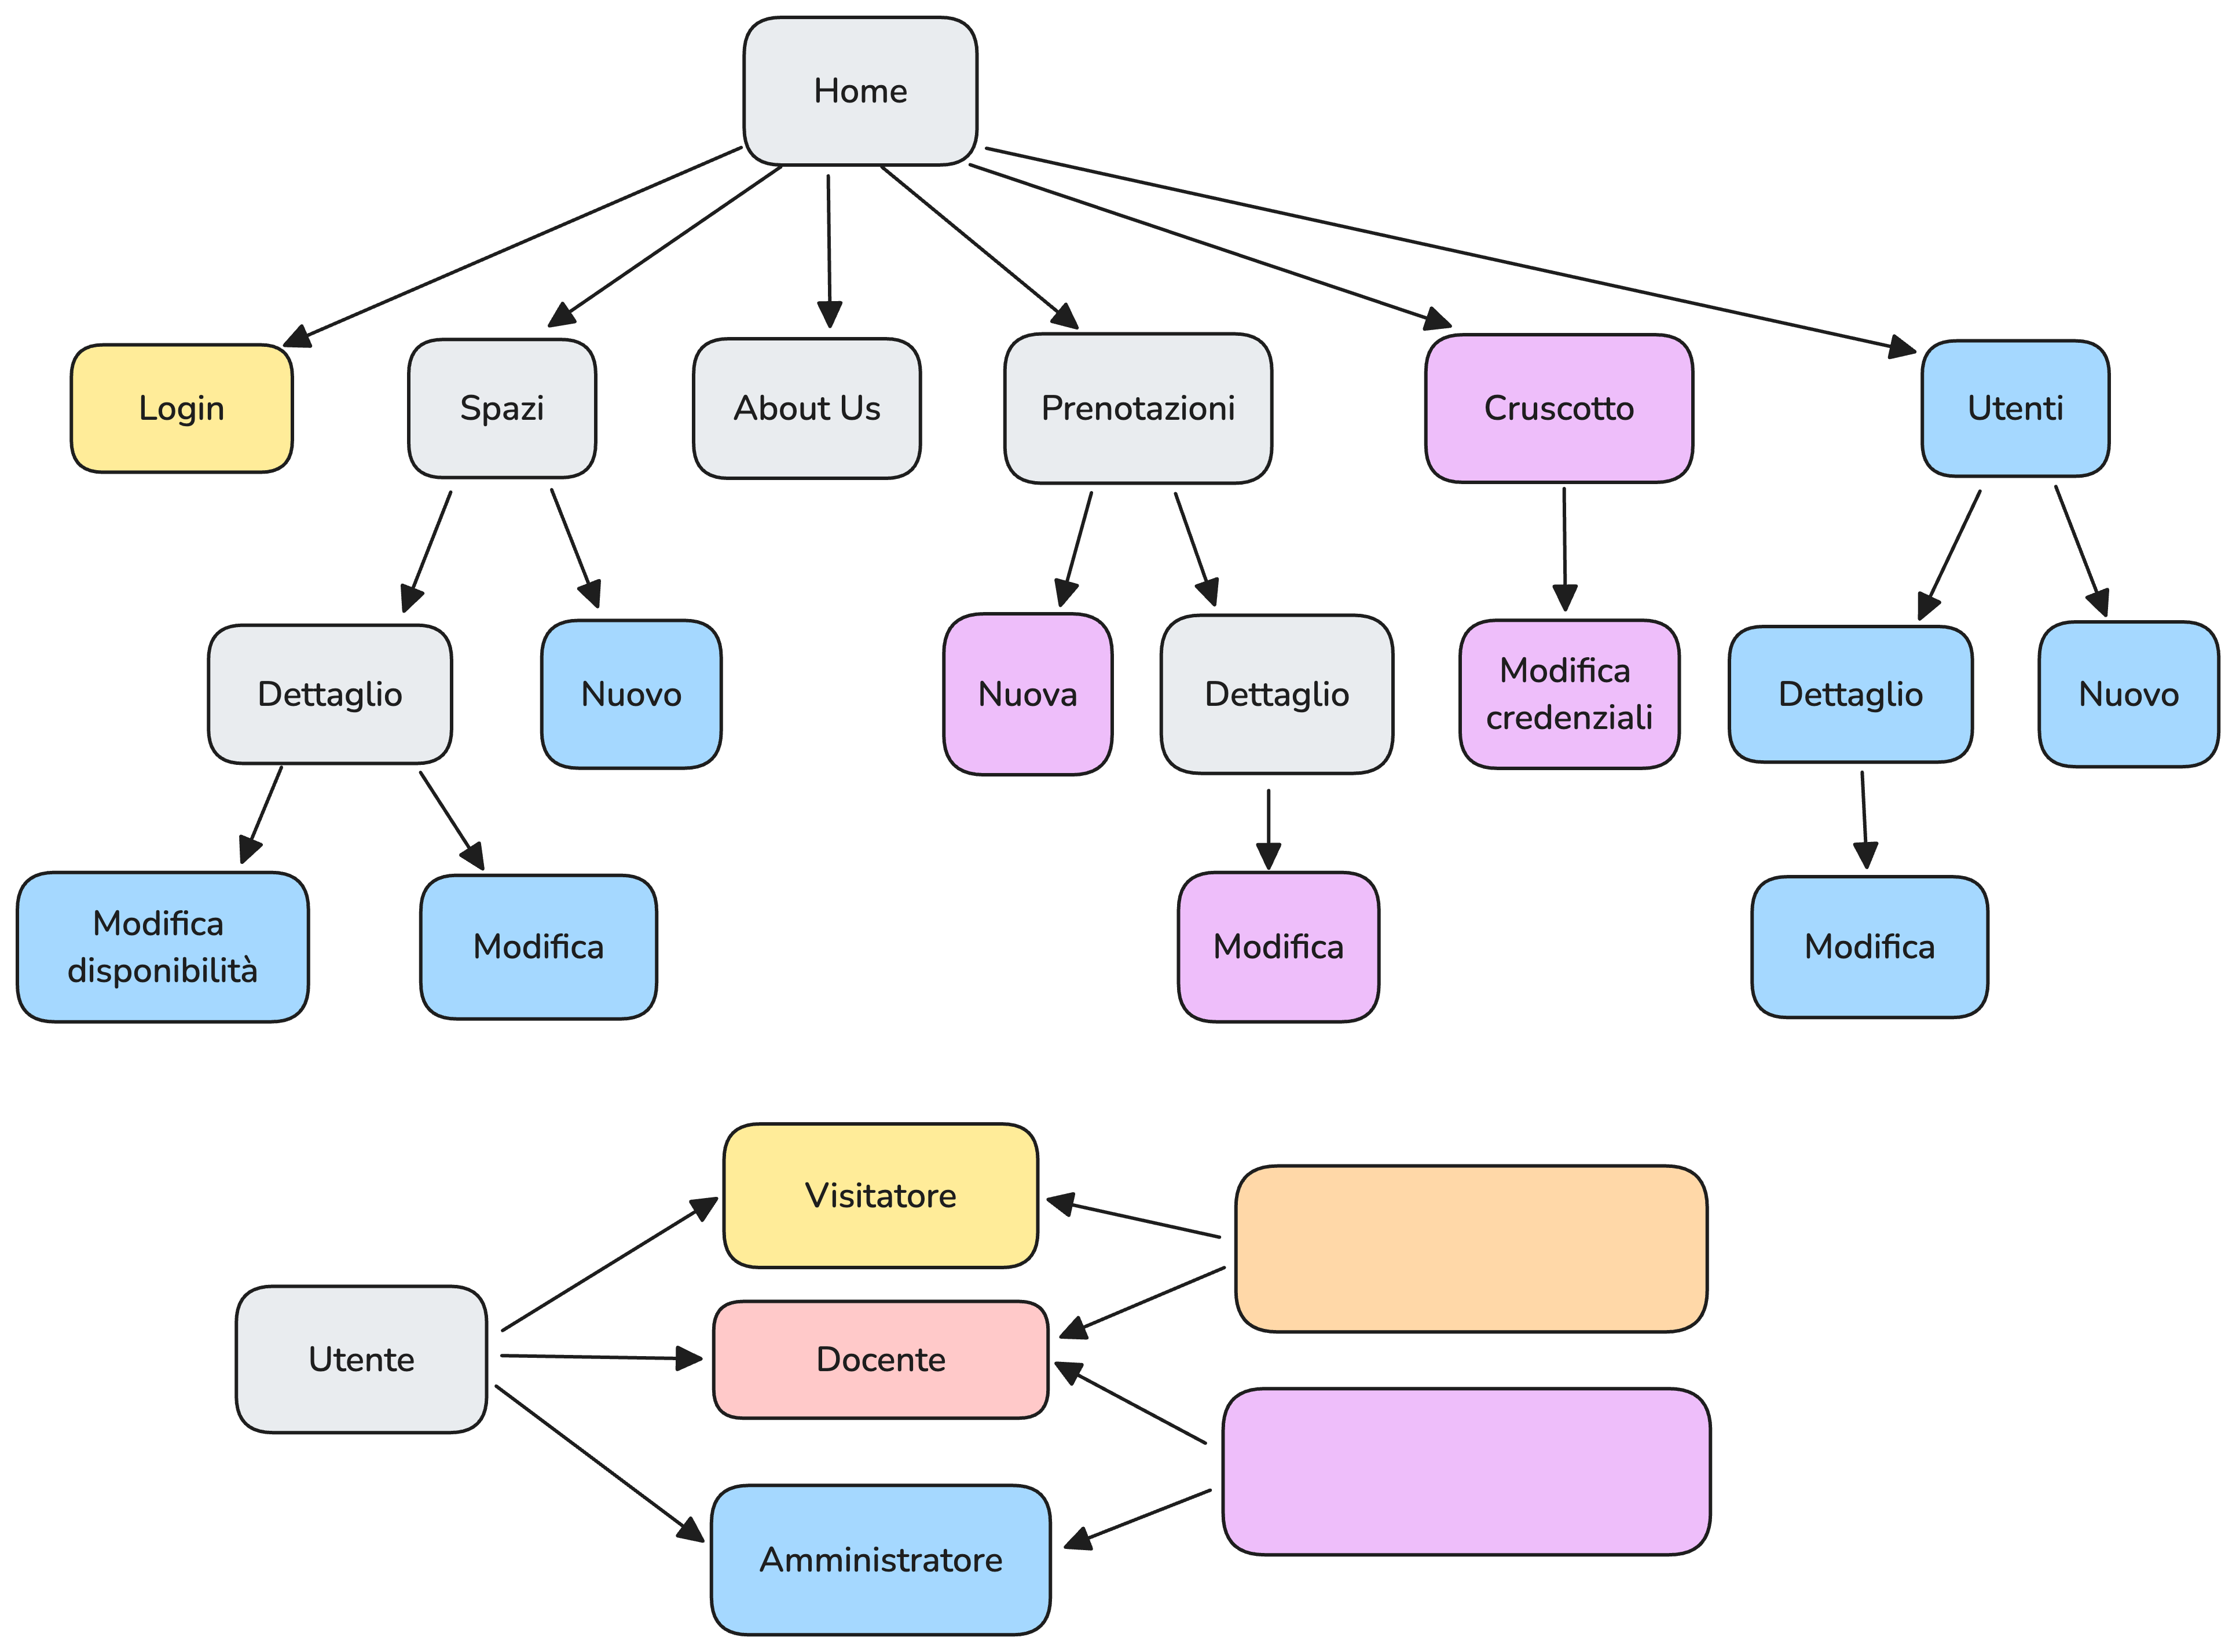
\includegraphics[width=0.8\textwidth]{figures/sitemap.png}
	\caption{Mappa del sito: i rettangoli rappresentano le pagine, le linee
		le connessioni tra le pagine, mentre gli ovali rappresentano le
		funzionalità. In basso a destra è spiegato l'uso dei colori.}
\end{figure}

Il sito è organizzato in una struttura gerarchica per conciliare facilità di
utilizzo e organizzazione delle informazioni in modo ordinato e preciso. I
contenuti sono suddivisi secondo uno schema organizzativo per argomento di
seguito sono descritte le singole pagine:

\begin{itemize}
	\item ...
\end{itemize}
